%% =====================================================================
%% Transactional Unit-Level NFC Shopping: A Concurrency-Safe
%% Tap-to-Cart Protocol -- IEEE conference format (IEEEtran)
%% Build: pdflatex nfc.tex (twice). nfc_results.tex is generated from
%% the benchmark harness (bench.py -> make_tables.py).
%% =====================================================================
\documentclass[conference]{IEEEtran}
\IEEEoverridecommandlockouts

\usepackage[T1]{fontenc}
\usepackage{cite}
\usepackage{amsmath,amssymb,amsfonts}
\usepackage{graphicx}
\usepackage{xcolor}
\usepackage{array}
\usepackage{booktabs}
\usepackage{tabularx}
\usepackage{listings}
\usepackage{tikz}
\usetikzlibrary{arrows.meta,positioning,calc}
\usepackage{pgfplots}
\pgfplotsset{compat=1.18}
\usepackage{xurl}
\usepackage[hidelinks]{hyperref}

\lstset{basicstyle=\ttfamily\scriptsize, breaklines=true, frame=tb,
  framerule=0.4pt, numbers=none, columns=fullflexible, keepspaces=true,
  showstringspaces=false, captionpos=b, aboveskip=4pt, belowskip=2pt,
  language=SQL, morekeywords={RETURNING,uuid,timestamptz,bigint,jsonb,ENUM,CONFLICT,SKIP,LOCKED}}

\newcommand{\Av}{\textsc{Available}}
\newcommand{\Rs}{\textsc{Reserved}}
\newcommand{\So}{\textsc{Sold}}
\input{nfc_results}
\input{nfc_tla}

\begin{document}

\title{Transactional Unit-Level NFC Shopping:\\
A Concurrency-Safe Tap-to-Cart Protocol}

\author{
\IEEEauthorblockN{Jeevan U Gowda}
\IEEEauthorblockA{\textit{Dept. of Information Science and Engineering}\\
\textit{B.M.S. College of Engineering}\\
Bengaluru, India\\
jeevanu342005@gmail.com}
\and
\IEEEauthorblockN{Mithun Krishna T}
\IEEEauthorblockA{\textit{Dept. of Information Science and Engineering}\\
\textit{B.M.S. College of Engineering}\\
Bengaluru, India}
\and
\IEEEauthorblockN{Sahana P}
\IEEEauthorblockA{\textit{Dept. of Information Science and Engineering}\\
\textit{B.M.S. College of Engineering}\\
Bengaluru, India}
\and
\IEEEauthorblockN{H S Guruprasad}
\IEEEauthorblockA{\textit{Dept. of Information Science and Engineering}\\
\textit{B.M.S. College of Engineering}\\
Bengaluru, India}
% AUTHORS: add the other authors' e-mail addresses (institutional addresses preferred).
}

\maketitle

\begin{abstract}
NFC lets shoppers tap tagged products with ordinary smartphones, but
little prior work specifies what happens when a tag identifies one
physical unit that several actors try to change at once. We specify a
tap-to-cart protocol in which reservation, release, expiry, checkout,
sale, and return are conditional atomic transitions guarded by
reservation ownership, a monotonic version, and idempotency keys, with
unit state kept separate from payment state so that no distributed
transaction is needed. A TLA$^{+}$ model explored exhaustively with
TLC (\TLAStates\ states) verifies nine safety properties, shows that
each guard except the version check is necessary, and exposed a
checkout-rebinding gap in our earlier draft, which we fixed. A
PostgreSQL prototype, over \NRuns\ runs, showed no violation in
\HotTotalRounds\ hot-unit rounds with up to 200 clients or in eleven
fault-injection scenarios, while an unguarded baseline double-reserved
in every contended round. The single conditional update sustained
\LowCUpeakX\ the peak throughput of \texttt{SELECT~FOR~UPDATE}, and
\RTTx\ with a 5~ms network round trip. We also separate what static
and authenticated NFC tags guarantee, and release a field-test kit for
measuring NFC read reliability.
\end{abstract}

\begin{IEEEkeywords}
Near Field Communication, item-level identification, concurrency
control, idempotency, inventory reservation, retail systems, NFC
security
\end{IEEEkeywords}

%% ---------------------------------------------------------------------
\section{Introduction}

Smartphones with NFC give shoppers a simple way to interact with
physical products. Earlier work has used NFC for shopping assistance,
product information, mobile commerce, and
payment~\cite{refCoskun,refHusni,refParadowski,refBroll,refDave,refJe}.
Individual-item identification is also well established through
serialized GS1 identifiers and item-level RFID
deployments~\cite{refGS1TDS,refChoi,refCilloni,refHou}. The open
question this paper addresses is therefore not whether an item can
carry its own identifier. It is how a tap on one serialized unit
should become a retail transaction that stays correct under
concurrency, retries, and partial failures.

Suppose a tag resolves to one inventory unit. While a shopper taps
it, another shopper may reserve the same unit, the phone may resend a
request, an expiry worker may reclaim it, and a checkout may be in
progress, while the external payment provider cannot commit
atomically with the retailer's database. A correct design must
prevent double reservation, stale updates, cross-session
finalization, and double sales, and must tolerate retries.

NFC shopping prototypes~\cite{refHusni,refParadowski,refBroll,refDave,refJe}
and item-level RFID systems~\cite{refHou,refChoi,refCilloni,refLi}
show that both smartphone interaction and serialized inventory are
feasible. In the work we reviewed, however, we found little that
specifies the transaction protocol behind a consumer NFC tap:
ownership, expiry, stale-write rejection, idempotency, concurrent
cleanup, and recovery from payment failures. This paper makes the
following contributions.
\begin{enumerate}
\item A unit-level inventory state model that separates the identity
of a physical unit from its product class and keeps unit state apart
from order and payment state.
\item A reservation and checkout protocol built from conditional
atomic updates, monotonic versions, reservation ownership, and
idempotency keys, with a failure model covering duplicated requests,
lost responses, competing cleanup workers, and the non-atomic payment
boundary.
\item A correctness argument under stated PostgreSQL transaction
assumptions, and a TLA$^{+}$ model checked exhaustively with TLC,
including negative controls that show each guard is necessary.
\item A PostgreSQL prototype evaluated over \NRuns\ runs for
contention, throughput, emulated network delay, and eleven
fault-injection scenarios, against a \texttt{SELECT~FOR~UPDATE}
implementation and an unguarded baseline.
\item A security analysis that distinguishes static NFC identification
from cryptographically authenticated NFC.
\end{enumerate}

%% ---------------------------------------------------------------------
\section{Related Work}
\label{sec:related}

\textbf{NFC shopping.}
Husni and Purwantoro built an Android shopping application around
NFC~\cite{refHusni}. Paradowski and Kr\"uger split mobile shopping
assistance into modules such as shopping list, basket, and
payment~\cite{refParadowski}, and Broll \emph{et al.} studied
multimodal feedback for NFC-tagged groceries~\cite{refBroll}. Dave
\emph{et al.} used product tags to add items to and remove them from a
mobile trolley~\cite{refDave}, and Je and Seo designed a smart-mall
platform around NFC-tagged products~\cite{refJe}. More recent IoT
smart carts automate checkout with RFID, weight sensing, or
cameras~\cite{refBatool,refWang}; they bill a basket but do not specify
what happens when two shoppers, a timer, and a payment callback act on
the same unit. NFC shopping as such is therefore not new.

\textbf{Item-level identification.}
GS1 identifies an individual trade item by a GTIN plus a serial
number, which EPC/SGTIN encodings carry in electronic
tags~\cite{refGS1TDS}. RFID-based shopping and apparel
systems~\cite{refHou,refChoi}, a review of item-level RFID in fashion
retail~\cite{refCilloni}, and a secure RFID smart-shopping
system~\cite{refLi} show that serialized retail tracking is
established practice. We do not claim it as a contribution.

\textbf{Concurrency control.}
Optimistic concurrency control~\cite{refKung} avoids locks when
conflicts are rare. Our protocol uses a related idea: each transition
is a single conditional update, similar to compare-and-swap, whose
predicate checks the expected state and version. Under PostgreSQL's
default Read Committed level, an \texttt{UPDATE} that meets a row
being changed by another transaction waits for it and then
re-evaluates its \texttt{WHERE} clause on the new row
version~\cite{refPGIsolation}. The protocol relies on this behavior.

In short, prior work covers tagged-product interaction and
serialized tracking, whereas this paper specifies and verifies the
transactional state of each serialized unit.

%% ---------------------------------------------------------------------
\section{System Model and Requirements}
\label{sec:model}

\textbf{Entities.}
A \emph{physical unit} is one sellable object. It carries an
\emph{NFC tag} holding a URI that resolves to the unit's identity. A
\emph{consumer client} (smartphone) calls a \emph{reservation service},
which is the authoritative API for reserving and releasing units. An
\emph{order service} coordinates checkout with an external
\emph{payment provider}. The \emph{inventory database} is the source
of truth for unit state, and \emph{background workers} handle expiry,
reconciliation, and event delivery (Fig.~\ref{fig:architecture}).

\textbf{Assumptions.}
(A1) All inventory mutations reach one authoritative PostgreSQL
database. (A2) Each atomic phase is one transaction, and callers check
the number of changed rows. (A3) Isolation is Read Committed or
stronger, with PostgreSQL's re-evaluation of \texttt{WHERE}
predicates on concurrently updated rows~\cite{refPGIsolation}.
(A4) The service authenticates sessions; a compromised backend is out
of scope. (A5) Leases use the database clock. (A6) Payment and
inventory never share an atomic commit. (A7) A static NDEF record
identifies a unit but does not prove that the tag is genuine or
attached to the right product. (A8) State changes require the backend
to be reachable.

\textbf{Requirements.}
(R1) \emph{Exclusivity}: at most one active reservation owns a unit.
(R2) \emph{Ownership}: only the owner releases or checks out.
(R3) \emph{Stale-write rejection}: an operation based on an old
version cannot overwrite newer state.
(R4) \emph{Sale uniqueness}: at most one sale per unit and sale epoch.
(R5) \emph{Retry safety}: a repeated request with the same key has no
further effect.
(R6) \emph{Reclaimability}: expired, unprotected reservations are
eventually reclaimable.
(R7) \emph{Payment recovery}: duplicates, lost responses, and crashes
never cause a second charge.

\begin{figure}[!t]
\centering
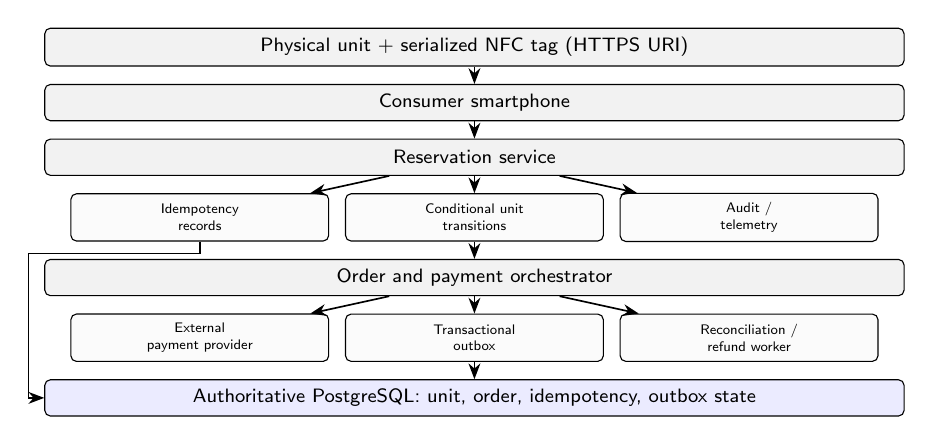
\begin{tikzpicture}[
  font=\scriptsize\sffamily, node distance=2.2mm,
  box/.style={draw, rounded corners=2pt, minimum width=0.9\columnwidth,
              minimum height=4.6mm, align=center, fill=gray!10},
  sb/.style={draw, rounded corners=2pt, minimum width=0.27\columnwidth,
             minimum height=6mm, align=center, fill=gray!3, font=\tiny\sffamily},
  arr/.style={-Stealth, semithick}]
\node[box] (phys) {Physical unit + serialized NFC tag (HTTPS URI)};
\node[box, below=of phys] (cli) {Consumer smartphone};
\node[box, below=of cli] (res) {Reservation service};
\node[sb, below=of res] (inv) {Conditional unit\\transitions};
\node[sb, left=2mm of inv] (idem) {Idempotency\\records};
\node[sb, right=2mm of inv] (aud) {Audit /\\telemetry};
\node[box, below=of inv] (ord) {Order and payment orchestrator};
\node[sb, below=of ord] (out) {Transactional\\outbox};
\node[sb, left=2mm of out] (pay) {External\\payment provider};
\node[sb, right=2mm of out] (rec) {Reconciliation /\\refund worker};
\node[box, below=of out, fill=blue!8] (db) {Authoritative PostgreSQL: unit, order, idempotency, outbox state};
\foreach \a/\b in {phys/cli, cli/res, res/inv, res/idem, res/aud, inv/ord, ord/out, ord/pay, ord/rec, out/db}
  \draw[arr] (\a) -- (\b);
\draw[arr] (idem.south) -- ++(0,-1.5mm) -| ([xshift=-2mm]ord.north west) |- (db.west);
\end{tikzpicture}
\caption{Protocol-centered architecture. Every state change commits in
the authoritative database; the payment provider sits outside that
transactional boundary.}
\label{fig:architecture}
\end{figure}

%% ---------------------------------------------------------------------
\section{Unit Identity and NFC Representation}
\label{sec:identity}

\textbf{Identifiers.}
The database key of a unit is a time-ordered UUIDv7, generated by
\texttt{uuidv7()} in PostgreSQL~18~\cite{refPGIsolation} or by the
application. A GS1 GTIN plus serial number (SGTIN)~\cite{refGS1TDS}
and a readable staff code may be stored alongside, but only the UUID
is used for uniqueness, avoiding counters coordinated across stores.

\textbf{NDEF size.}
The tag stores an HTTPS URI that resolves to the unit, for example the 64-character URI
\begin{center}\footnotesize
\url{https://store.example.com/u/019535d9-3df7-79fb-b466-fa907fa17f9e}
\end{center} NDEF URI records replace the \texttt{https://} prefix
with a single code byte~\cite{refNFCNDEF}, leaving a
57-byte payload. A short record adds a header, type-length,
payload-length, and type byte, giving 61 bytes. The Type~2 TLV wrapper
(type, length, terminator) brings the total to 64 bytes, which leaves
80 of the 144 user bytes of an NTAG213 free.

\textbf{Tags.}
NTAG213/215/216 are passive NFC Forum Type~2 tags with 144, 504, and
888 user bytes, 13.56~MHz operation, 106~kbit/s, an operating distance
of up to 100~mm depending on the reader, 10-year data retention, and
100{,}000 write cycles~\cite{refNTAG21x}; the interaction is therefore
centimeter-scale.

\textbf{Provisioning and DPP.}
Tags are written in batches, read back and compared with the
manifest, locked or password-protected, and only then attached.
Read-back catches encoding errors but cannot prove that a tag stays
on its product. Regulation (EU) 2024/1781 lets delegated acts choose
the data carrier of a Digital Product Passport, at model, batch, or
item level, without mandating NFC~\cite{refESPR}; the NFC Forum has
specified how NFC tags carry passport links~\cite{refNFCDPP}.

%% ---------------------------------------------------------------------
\section{Transaction Protocol}
\label{sec:protocol}

Fig.~\ref{fig:sequence} gives the complete flow from tap to sale; the
rest of this section specifies each step.


\begin{figure}[!t]
\centering
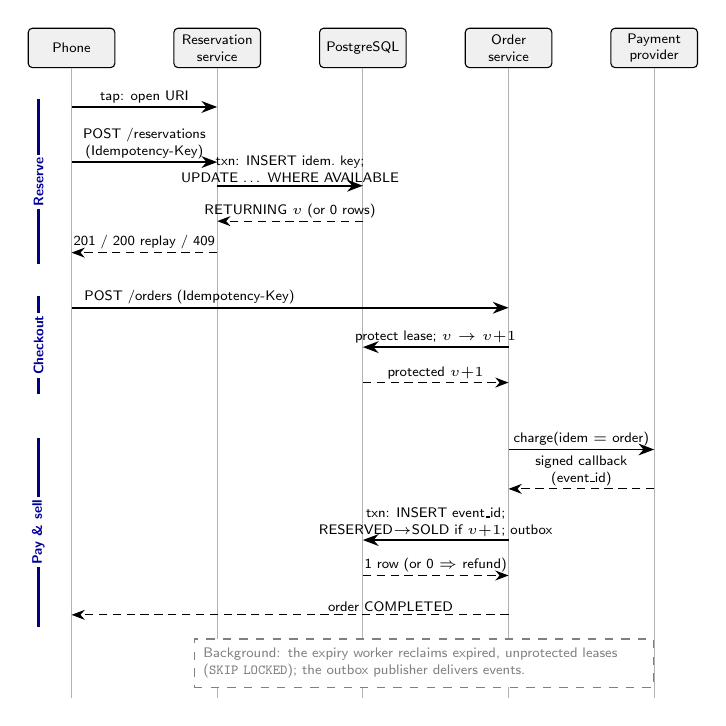
\begin{tikzpicture}[font=\tiny\sffamily, >=Stealth,
  hd/.style={draw, rounded corners=1.5pt, fill=gray!12, minimum width=11mm,
             minimum height=5mm, align=center, inner sep=1.5pt},
  msg/.style={->, semithick},
  ret/.style={->, densely dashed},
  lb/.style={above, inner sep=1pt, align=center},
  act/.style={draw, fill=blue!8, minimum width=1.6mm, inner sep=0pt}]
\def\xa{0}\def\xb{1.85}\def\xc{3.7}\def\xd{5.55}\def\xe{7.4}
\foreach \x/\n/\t in {\xa/a/Phone, \xb/b/Reservation\\service, \xc/c/PostgreSQL,
                      \xd/d/Order\\service, \xe/e/Payment\\provider}{
  \node[hd] (\n) at (\x,0) {\t};
  \draw[gray!60] (\n.south) -- (\x,-8.25);}
% phase labels
\foreach \ya/\yb/\t in {-0.65/-2.75/Reserve, -3.15/-4.4/Checkout, -4.95/-7.35/Pay \& sell}{
  \draw[blue!50!black, thick] (-0.42,\ya) -- (-0.42,\yb);
  \node[rotate=90, font=\tiny\bfseries\sffamily, text=blue!60!black, fill=white, inner sep=1pt]
    at (-0.42,{(\ya+\yb)/2}) {\t};}
% reserve
\draw[msg] (\xa,-0.75) -- node[lb] {tap: open URI} (\xb,-0.75);
\draw[msg] (\xa,-1.45) -- node[lb] {POST /reservations\\(Idempotency-Key)} (\xb,-1.45);
\draw[msg] (\xb,-1.75) -- node[lb] {txn: INSERT idem.\ key;\\UPDATE \ldots\ WHERE AVAILABLE} (\xc,-1.75);
\draw[ret] (\xc,-2.2) -- node[lb] {RETURNING $v$\ (or 0 rows)} (\xb,-2.2);
\draw[ret] (\xb,-2.6) -- node[lb] {201 / 200 replay / 409} (\xa,-2.6);
% checkout
\draw[msg] (\xa,-3.3) -- node[lb, pos=0.27] {POST /orders (Idempotency-Key)} (\xd,-3.3);
\draw[msg] (\xd,-3.8) -- node[lb] {protect lease; $v \to v{+}1$} (\xc,-3.8);
\draw[ret] (\xc,-4.25) -- node[lb] {protected $v{+}1$} (\xd,-4.25);
% pay & sell
\draw[msg] (\xd,-5.1) -- node[lb] {charge(idem $=$ order)} (\xe,-5.1);
\draw[ret] (\xe,-5.6) -- node[lb] {signed callback\\(event\_id)} (\xd,-5.6);
\draw[msg] (\xd,-6.25) -- node[lb] {txn: INSERT event\_id;\\RESERVED$\to$SOLD if $v{+}1$; outbox} (\xc,-6.25);
\draw[ret] (\xc,-6.7) -- node[lb] {1 row (or 0 $\Rightarrow$ refund)} (\xd,-6.7);
\draw[ret] (\xd,-7.2) -- node[lb, pos=0.27] {order COMPLETED} (\xa,-7.2);
\node[draw, dashed, gray, fill=white, align=left, anchor=north west, font=\tiny\sffamily,
      text width=56mm] at (\xb-0.3,-7.5)
 {Background: the expiry worker reclaims expired, unprotected leases
 (\texttt{SKIP LOCKED}); the outbox publisher delivers events.};
\end{tikzpicture}
\caption{End-to-end flow from tap to sale. Solid arrows are requests,
dashed arrows are responses. Every state change is a conditional
update that commits together with its idempotency or event record.}
\label{fig:sequence}
\end{figure}

\subsection{Two Separate State Machines}

A unit can be reserved, released or expired, finalized, and returned
(Fig.~\ref{fig:states}). Payment does not appear in the unit's life
cycle; orders follow their own machine: \textsc{Created} $\to$
\textsc{PaymentPending} $\to$ \textsc{Paid} $\to$ \textsc{Completed},
with branches to \textsc{PaymentFailed} and to
\textsc{RefundPending} $\to$ \textsc{Refunded}. The
\texttt{inventory\_unit} table is the only source of availability; any
stock counter is a derived projection.

\begin{figure}[!t]
\centering
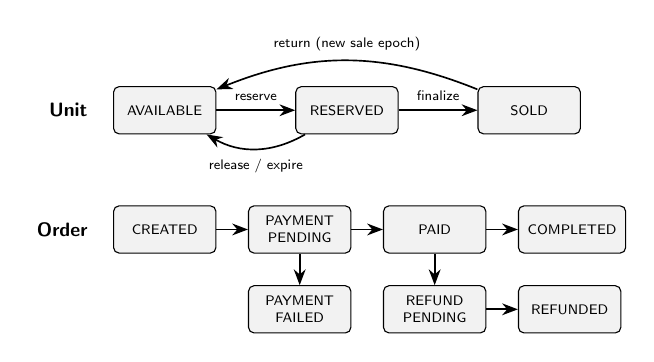
\begin{tikzpicture}[
  font=\tiny\sffamily, node distance=7mm and 4mm,
  st/.style={draw, rounded corners=2pt, minimum width=13mm, minimum height=6mm,
             align=center, fill=gray!10},
  arr/.style={-Stealth, semithick}]
\node[st] (a) {AVAILABLE};
\node[st, right=10mm of a] (r) {RESERVED};
\node[st, right=10mm of r] (s) {SOLD};
\draw[arr] (a) -- node[above] {reserve} (r);
\draw[arr] (r) -- node[above] {finalize} (s);
\draw[arr] (r) to[bend left=30] node[below] {release / expire} (a);
\draw[arr] (s) to[bend right=22] node[above] {return (new sale epoch)} (a);
\node[st, below=9mm of a] (c) {CREATED};
\node[st, right=of c] (p) {PAYMENT\\PENDING};
\node[st, right=of p] (pd) {PAID};
\node[st, right=of pd] (cm) {COMPLETED};
\node[st, below=4mm of p] (f) {PAYMENT\\FAILED};
\node[st, below=4mm of pd] (rf) {REFUND\\PENDING};
\node[st, right=of rf] (rd) {REFUNDED};
\draw[arr] (c)--(p); \draw[arr] (p)--(pd); \draw[arr] (pd)--(cm);
\draw[arr] (p)--(f); \draw[arr] (pd)--(rf); \draw[arr] (rf)--(rd);
\node[anchor=east, font=\scriptsize\bfseries\sffamily] at ([xshift=-2mm]a.west) {Unit};
\node[anchor=east, font=\scriptsize\bfseries\sffamily] at ([xshift=-2mm]c.west) {Order};
\end{tikzpicture}
\caption{Unit and order state machines are kept separate.}
\label{fig:states}
\end{figure}

\subsection{Data Model}

Listing~\ref{lst:schema} shows the core table. The \texttt{CHECK}
constraint makes the database itself reject any row whose fields do
not match its state, so a buggy code path cannot, for example, leave a
\So\ unit with an owner. Separate tables hold orders, the
\texttt{order\_unit} binding (with the version protected at checkout),
idempotency records keyed by \texttt{(operation\_scope, key)},
payment events keyed by the provider's event identifier, and outbox
events.

\begin{lstlisting}[caption={Core unit table (abridged).}, label={lst:schema}]
CREATE TABLE inventory_unit (
  unit_id uuid PRIMARY KEY DEFAULT uuidv7(),
  sku_id text NOT NULL REFERENCES product,
  status unit_status NOT NULL DEFAULT 'AVAILABLE',
  reservation_id uuid, owner_session_id uuid,
  reserved_until timestamptz,
  checkout_order_id uuid REFERENCES customer_order,
  checkout_protected_until timestamptz,
  sold_order_id uuid REFERENCES customer_order,
  sold_at timestamptz,
  sale_epoch int NOT NULL DEFAULT 0,
  version bigint NOT NULL DEFAULT 0,
  CHECK (
    (status='AVAILABLE' AND reservation_id IS NULL
     AND owner_session_id IS NULL
     AND sold_order_id IS NULL)
    OR (status='RESERVED'
     AND reservation_id IS NOT NULL
     AND owner_session_id IS NOT NULL
     AND sold_order_id IS NULL)
    OR (status='SOLD' AND reservation_id IS NULL
     AND sold_order_id IS NOT NULL)),
  CHECK (checkout_order_id IS NULL
         OR status='RESERVED'));
\end{lstlisting}

\textbf{API.}
\texttt{POST /v1/reservations} and \texttt{POST /v1/orders} require
an \texttt{Idempotency-Key} header. A reservation returns 201 when
new, 200 for a replay, and 409 when the unit is not available.
\texttt{DELETE /v1/reservations/\{id\}} releases an owned reservation.
Payment failures are reported in the order resource (e.g.,
\texttt{"status":"PAYMENT\_FAILED"}), not through HTTP~402, which
RFC~9110 reserves for future use~\cite{refRFC9110}.

\subsection{Reservation}

A reservation is one conditional update (Listing~\ref{lst:reserve}).
It succeeds if and only if a row is returned; \texttt{RETURNING}
gives the new version without a second query~\cite{refPGIsolation}.

\begin{lstlisting}[caption={Atomic reservation.}, label={lst:reserve}]
UPDATE inventory_unit
SET status='RESERVED', reservation_id=:rid,
    owner_session_id=:sid, reserved_until=now()+:ttl,
    version=version+1
WHERE unit_id=:uid AND status='AVAILABLE'
RETURNING version, reserved_until;
\end{lstlisting}

If two requests race, the second waits for the first and then
re-checks \texttt{status='AVAILABLE'} against the committed row, which
is now \Rs, so it updates nothing~\cite{refPGIsolation}. The
successful update is the operation's linearization point.

\textbf{Idempotency.}
In the same transaction as the update, the service first executes
\texttt{INSERT INTO idempotency\_record \ldots\ ON CONFLICT DO NOTHING}
with the key and a hash of the request. If the insert returns no row,
another request with the same key already exists. The unique index
makes a concurrent duplicate wait until the first transaction
commits; the duplicate then returns the stored response, or is
rejected if its request hash differs. Because the record and the
state change commit together, a crash can never leave one without the
other. The reservation UUID names the resulting lease, whereas the
idempotency key names one logical API call.

\subsection{Release and Expiry}

Release uses the same pattern, with the predicate
\texttt{status='RESERVED' AND reservation\_id=:rid AND
owner\_session\_id=:sid AND version=:v}, and additionally requires that
no checkout protection is active
(\texttt{checkout\_order\_id IS NULL OR checkout\_protected\_until
<= now()}). A cart removal therefore cannot undo a checkout in
progress.

An expiry worker reclaims leases with
\texttt{reserved\_until <= now()} whose checkout protection is absent
or expired. It processes batches selected with
\texttt{FOR UPDATE SKIP LOCKED}, so parallel workers take disjoint
rows instead of queuing on the same ones (Section~\ref{sec:eval}).
Once one worker resets a row to \Av, the predicate of any competing
worker is false. Reclamation is a liveness property: an expired,
unprotected reservation becomes available \emph{provided that} some
worker keeps running. The reservation transition could also accept
expired, unprotected \Rs\ rows directly, which would remove the
dependence on the worker for availability.

\subsection{Checkout, Payment, and Sale}

\textbf{Checkout preparation.}
In one local transaction, the order service creates or loads the
order idempotently, and for every unit checks ownership and the
expected version, refuses to rebind a unit whose checkout protection
for another order is still active (\texttt{checkout\_order\_id IS NULL
OR checkout\_protected\_until <= now()}), sets
\texttt{checkout\_order\_id} and a bounded
\texttt{checkout\_protected\_until}, increments the version, and stores
the new version in \texttt{order\_unit}. If any unit fails, the whole
transaction rolls back. The bounded lease keeps the expiry worker away
during a normal payment without locking the unit forever if the
orchestrator fails. Model checking showed why the rebinding guard is
needed (Section~\ref{sec:tla}): without it, a client that has learned
the latest version can start a second order for the same reservation
and move the unit away from an order whose payment is in flight.

\textbf{Payment boundary.}
After this commit, the payment provider is called with a stable
idempotency identifier derived from the order. Callbacks are
authenticated and deduplicated by inserting the provider's event
identifier into a table with a unique key. A lost response therefore
never triggers a second charge; the service looks up the existing
payment attempt instead. A successful payment moves the order to
\textsc{Paid}, after which a reconciliation worker may retry
finalization safely.

\textbf{Sale finalization.}
Listing~\ref{lst:sale} moves each unit to \So, guarded by the
reservation, the order binding, and the protected version. All units
of an order are finalized in one transaction.

\begin{lstlisting}[caption={Conditional sale finalization.}, label={lst:sale}]
UPDATE inventory_unit
SET status='SOLD', sold_order_id=:oid, sold_at=now(),
    reservation_id=NULL, owner_session_id=NULL,
    reserved_until=NULL, checkout_order_id=NULL,
    checkout_protected_until=NULL, version=version+1
WHERE unit_id=:uid AND status='RESERVED'
  AND reservation_id=:rid AND checkout_order_id=:oid
  AND version=:protected_version
RETURNING version, sold_at;
\end{lstlisting}

If payment succeeded but a unit can no longer be finalized (for
instance, a long database outage let its lease expire and the unit
was legitimately reclaimed and resold), the customer is not charged
again. The order enters an idempotent refund or manual-review path.

\textbf{Returns.}
A return is the only transition out of \So. It is a conditional update
(\texttt{WHERE status='SOLD' AND sold\_order\_id=:oid AND
version=:v}) that resets the unit to \Av\ and increments a
\texttt{sale\_epoch} column. Each sale is also inserted into a
\texttt{unit\_sale} table whose primary key is
\texttt{(unit\_id, sale\_epoch)}, so the database itself rejects a
second sale within an epoch, and the sales history survives the
reset. Sale uniqueness therefore holds per epoch (R4).

\textbf{Transactional outbox.}
Events such as \texttt{InventorySold} are written to an outbox table
in the same transaction as the state change and published
asynchronously. A failure after commit but before publication leaves
an unpublished row that is retried later; the committed sale is never
rolled back.

%% ---------------------------------------------------------------------
\section{Correctness Properties}
\label{sec:correctness}

For each unit $u$ let $\mathit{st}(u)\in\{\Av,\Rs,\So\}$, with owner,
reservation, and sold-order fields that are either set or $\bot$, and a
version $v(u)\in\mathbb{N}$. The \texttt{CHECK} constraints enforce:
\emph{I1}, $\mathit{st}(u)=\Rs \Rightarrow$ reservation and owner are
set; \emph{I2}, $\mathit{st}(u)\neq\Rs \Rightarrow$ both are $\bot$;
and \emph{I3}, $\mathit{st}(u)=\So \Rightarrow$ the sold order is set.
Every successful transition increments $v(u)$ by one (\emph{I4}).

\textbf{Exclusivity (R1).}
Let $T_1$ and $T_2$ run Listing~\ref{lst:reserve} on an \Av\ unit. If
$T_1$ updates the row first, $T_2$ blocks on the row lock. Under A3,
when $T_1$ commits, $T_2$ re-evaluates its predicate on the new row
version~\cite{refPGIsolation}; since $\mathit{st}(u)=\Rs$, the
predicate is false and $T_2$ updates nothing. If $T_1$ aborts, $T_2$
proceeds on the unchanged row. Either way at most one reservation
succeeds, and by I2 a unit can only become reservable again through a
transition that clears its owner.

\textbf{Stale writes (R3).}
If an operation read version $v$, any intervening successful
transition makes the version at least $v+1$ (I4). A later update with
the predicate \texttt{version=$v$} then affects zero rows.

\textbf{Sale uniqueness (R4).}
Concurrent finalizations of the same unit are possible, but once one
succeeds the unit is \So\ with a new version, so the others fail both
the status and the version conditions. The only transition out of
\So\ is a return, which starts a new sale epoch, so at most one sale
per unit and epoch is possible.

\textbf{Ownership (R2) and retries (R5).}
Release and checkout predicates include the reservation identifier and
owning session, so knowing a unit's identifier is not enough to
release or buy another shopper's reservation. Retries resolve against
the unique idempotency or payment-event key rather than re-executing,
and a reused key with a different request hash is rejected.

These are safety properties: they hold whenever A1--A3 hold. R6 is a
liveness property and also requires the database and some expiry
worker to make progress.

\subsection{Model Checking with TLA\texorpdfstring{$^{+}$}{+}}
\label{sec:tla}

We encoded the protocol in TLA$^{+}$~\cite{refLamportTLA}, one atomic
action per database transition. Clients may act on \emph{any} version
they have observed (stale requests), and duplicates, timeouts, expiry,
charge retries, duplicate callbacks, finalization retries, and returns
interleave freely. The model has two sessions,
three orders (two belonging to the same session), up to
\TLAMaxRes\ reservations, and one unit. TLC~\cite{refTLC} checks five
state invariants (structural constraints I1--I3, at most one sale per
unit and epoch, no sale without a processed payment, at most one
charge per order, consistent completed and refunded orders) and four
action properties (reservation exclusivity, owner-only release,
version monotonicity, and that a unit under checkout protection is
never freed or rebound).

Table~\ref{tab:tla} reports the results. The protocol as specified
satisfies all properties over \TLAStates\ distinct states; a bounded
run with two units explored 21.5 million distinct states without a
violation before we stopped it. Each
negative control removes one guard and yields a counterexample. The
\emph{draft} variant, our earlier protocol without the rebinding
guard, violates protection: a session checks out the same reservation
twice, using the version returned by the first checkout. Removing the
version predicate alone produced no violation once reservation
identifiers are unique and the rebinding guard is present; the
version still gives cheap stale-write rejection and remains in the
protocol.

\begin{table}[!t]
\caption{TLC Results (One Unit, Two Sessions, Three Orders)}
\label{tab:tla}
\centering
\scriptsize
\setlength{\tabcolsep}{3pt}
\begin{tabularx}{\columnwidth}{@{}>{\raggedright\arraybackslash}p{3.0cm}>{\raggedright\arraybackslash}X r@{}}
\toprule
\textbf{Variant} & \textbf{Result} & \textbf{States}\\
\midrule
\TLARows
\bottomrule
\end{tabularx}
\end{table}

%% ---------------------------------------------------------------------
\section{Security and Trust}
\label{sec:security}

\textbf{Static Type~2 tags.}
NTAG21x tags support password-protected writes, lock bits, and an
originality signature~\cite{refNTAG21x}. These features resist
\emph{modification} of the tag, but a static NDEF URI can still be
copied to another tag. A static tag therefore identifies a database
record; it does not prove that the shopper is holding that product.

\textbf{Authenticated tags.}
NTAG~424~DNA adds AES-128 mutual authentication and Secure Unique NFC
(SUN) messages, in which each tap produces a fresh, counter-based
MAC~\cite{refNTAG424,refNTAG424App}. With properly managed keys and
server-side counter checks, a copied payload is rejected because it
cannot produce a new valid MAC. This reduces, but does not eliminate,
cloning risk: security still depends on key management and backend
validation. The TagTamper variant can report whether its tamper loop
is broken~\cite{refNTAG424}, but no tag proves that a label was never
moved from one product to another.

\textbf{Threat controls.}
NDEF rewriting is prevented by locking or password-protected writes
and validation of the URI origin. Static cloning and tap replay are
addressed only by authenticated tags with fresh counter-based
messages; tag swapping is detected by tamper-evident labels and checks
at fulfillment. Reservation flooding is limited by authenticated
sessions, quotas, rate limits, and short leases; duplicate checkouts
and callback replays are absorbed by idempotency keys, provider
signatures, and unique event identifiers; broken authorization is
prevented because every predicate includes the owner. Ordinary web
controls (TLS, HSTS, Secure/HttpOnly/SameSite cookies, CSRF tokens,
output encoding, and a Content Security Policy) apply as usual. The
protocol's session and order telemetry should be minimized, access
controlled, and retained only as long as legally required.

%% ---------------------------------------------------------------------
\section{Experimental Evaluation}
\label{sec:eval}

We implemented the protocol on PostgreSQL to test whether the safety
properties hold under real concurrency, and to measure what the
single-statement design costs or saves. This evaluation covers the
database protocol only; NFC read reliability and usability are
discussed in Section~\ref{sec:future}.

\subsection{Setup}

The prototype uses the schema of Listing~\ref{lst:schema} on
PostgreSQL~\PGversion\ (Read Committed,
\texttt{synchronous\_commit=on}, \texttt{max\_connections=600}). Since
this version lacks \texttt{uuidv7()}, keys are generated with
\texttt{gen\_random\_uuid()}, which does not affect the protocol. The
load generator is Python~\PYversion\ with psycopg~\PSYversion; each
client thread holds its own connection over a Unix socket. Server and
clients share one cloud VM with \textbf{2~vCPUs} and 8~GB of RAM, so
absolute numbers are conservative and the comparison between
implementations is what matters. Each configuration was run
\NRuns\ times; we report the mean $\pm$ standard deviation across
runs.

We compare three reservation implementations:
\emph{CU}, the conditional update of Listing~\ref{lst:reserve};
\emph{SFU}, a transaction that reads the row with
\texttt{SELECT~\ldots~FOR~UPDATE}, checks the status in the
application, and then updates it; and \emph{Naive}, a read without a
lock followed by an unconditional update. Naive is a negative control
that shows what the tests can detect.

\subsection{Hot-Unit Contention}

All $N\in\{1,10,50,100,200\}$ clients start together, behind a
barrier, and try to reserve the \emph{same} unit. We reset the unit
and repeat for 100 rounds ($N\le50$) or 40 rounds ($N\ge100$) per
run, \HotTotalRounds\ rounds per implementation in total. A round is \emph{oversold} if more than one client is told it
holds the unit. Table~\ref{tab:hot} shows the results.

\begin{table}[!t]
\caption{Hot-Unit Contention: Oversold Rounds and Median Request
Latency without and with a 5~ms Emulated Round Trip}
\label{tab:hot}
\centering
\scriptsize
\setlength{\tabcolsep}{3pt}
\setlength{\tabcolsep}{2.2pt}
\begin{tabular}{@{}r ccc cc cc@{}}
\toprule
& \multicolumn{3}{c}{\textbf{Oversold rounds}} & \multicolumn{2}{c}{\textbf{p50 (ms), 0 ms RTT}} & \multicolumn{2}{c}{\textbf{p50, 5 ms}}\\
\cmidrule(lr){2-4}\cmidrule(lr){5-6}\cmidrule(l){7-8}
$N$ & CU & SFU & Naive & CU & SFU & CU & SFU\\
\midrule
\HotRows
\bottomrule
\end{tabular}
\end{table}

CU and SFU never oversold the unit in any round of any run. The Naive
baseline oversold it in \emph{every} round with $N\ge10$, telling
\NaiveAvgFifty\ clients on average that they held the same unit at
$N=50$. CU is also markedly faster under contention: its median
latency at $N=200$ is \HotCUpFiftyTwoH~ms versus \HotSFUpFiftyTwoH~ms
for SFU. SFU holds a row lock across two round trips and an
application-side check, so waiting clients queue behind it, whereas CU
holds the lock only for the duration of one statement.

\subsection{Low-Contention Throughput}

Here each client repeatedly reserves randomly chosen units from a pool
of 300{,}000 for 8~s. Conflicts occur only when a client happens to
pick an already reserved unit. Fig.~\ref{fig:low} shows throughput and
p95 latency. CU peaks at \LowCUpeak$\pm$\LowCUpeakSD\ reservations/s
and SFU at \LowSFUpeak$\pm$\LowSFUpeakSD, a factor of \LowCUpeakX. Both decline beyond 50 clients
because the two vCPUs are shared by the server and all client threads.
In every run, the number of rows left in \Rs\ equaled the number of
successful reservations reported to clients, so no update was lost
and no success was reported for a row that was not changed.

\begin{figure}[!t]
\centering
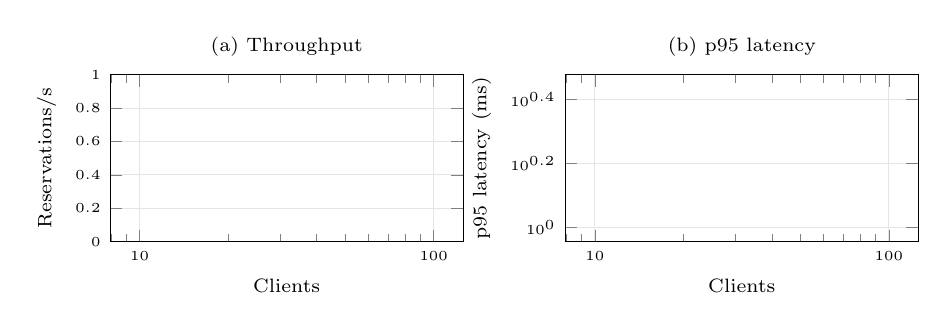
\begin{tikzpicture}
\begin{axis}[name=a1, width=0.5\columnwidth, height=3.7cm,
  xmode=log, log basis x=10, xtick={1,10,100}, xticklabels={1,10,100},
  xlabel={Clients}, ylabel={Reservations/s},
  ymin=0, ymax=8200, scaled y ticks=false,
  yticklabel style={/pgf/number format/fixed, /pgf/number format/1000 sep={}},
  tick label style={font=\tiny}, label style={font=\scriptsize},
  grid=major, grid style={gray!20},
  legend style={font=\tiny, at={(0.5,0.98)}, anchor=north, draw=gray!50, legend columns=2},
  title={(a) Throughput}, title style={font=\scriptsize, yshift=-1mm}]
\addplot[blue!80!black, thick, mark=*, mark size=1.3pt, error bars/.cd, y dir=both, y explicit] coordinates {\LowCUtput};
\addlegendentry{CU}
\addplot[red!75!black, thick, mark=square*, mark size=1.3pt, error bars/.cd, y dir=both, y explicit] coordinates {\LowSFUtput};
\addlegendentry{SFU}
\end{axis}
\begin{axis}[at={(a1.east)}, anchor=west, xshift=13mm, width=0.5\columnwidth, height=3.7cm,
  xmode=log, log basis x=10, xtick={1,10,100}, xticklabels={1,10,100},
  ymode=log, xlabel={Clients}, ylabel={p95 latency (ms)},
  tick label style={font=\tiny}, label style={font=\scriptsize},
  grid=major, grid style={gray!20},
  title={(b) p95 latency}, title style={font=\scriptsize, yshift=-1mm}]
\addplot[blue!80!black, thick, mark=*, mark size=1.3pt] coordinates {\LowCUpNinetyFive};
\addplot[red!75!black, thick, mark=square*, mark size=1.3pt] coordinates {\LowSFUpNinetyFive};
\end{axis}
\end{tikzpicture}
\caption{Random-unit reservation workload (mean over \NRuns\ runs;
error bars show $\pm$1 SD; 2-vCPU server and clients on one host).}
\label{fig:low}
\end{figure}

\subsection{Emulated Network Delay}

A deployment separates application and database by a network. We
repeated both workloads with a 5~ms round trip added to every
statement on the client (\NRTTRuns\ runs). SFU needs four round trips
per reservation and holds the row lock across three of them; CU needs
one. Under hot-unit contention at $N=200$, the median latency rises to
\RTTHotCU~ms for CU but \RTTHotSFU~ms for SFU
(Table~\ref{tab:hot}, last columns), and on random units with 200
clients CU sustains \RTTx\ the throughput of SFU. Neither oversold
(\RTTOversold\ rounds), while Naive oversold in \RTTnaiveRounds\
contended rounds.

\subsection{Fault Injection and Race Scenarios}

Table~\ref{tab:faults} lists the scenarios. Each targets one
requirement and checks the final database state rather than only the
responses.

\begin{table}[!t]
\caption{Fault-Injection and Race Scenarios}
\label{tab:faults}
\centering
\scriptsize
\renewcommand{\arraystretch}{1.08}
\begin{tabularx}{\columnwidth}{@{}>{\raggedright\arraybackslash}p{2.95cm}>{\centering\arraybackslash}p{0.95cm}>{\raggedright\arraybackslash}X@{}}
\toprule
\textbf{Scenario} & \textbf{Req.} & \textbf{Observed}\\
\midrule
\FaultRows
\bottomrule
\end{tabularx}
\end{table}

Two results deserve comment. In F5, checkout preparation and expiry
race on a lease that has just expired. Each race had exactly one
winner, and the final state matched it: units that checkout won were
protected, and units that expiry won were \Av. Which side wins
depends on timing, and either outcome is acceptable as long as it is
exclusive. In F4, the plain batched expiry query was correct but
serialized: workers queued on rows locked by another worker and then
found nothing left, and in \FourSingle\ of \NRuns\ runs a single worker
reclaimed all 20{,}000 leases. With \texttt{FOR UPDATE SKIP LOCKED},
all eight workers took disjoint batches and the 20{,}000 leases were
reclaimed in \FourSkipSec~s on average, with the same correctness.

\textbf{Threats to validity.}
Passing tests are evidence, not proof, which is why
Sections~\ref{sec:correctness} and~\ref{sec:tla} argue and model-check
the properties. The 2-vCPU host compresses absolute throughput, the
delay is emulated, and the results assume PostgreSQL Read Committed
semantics; replicated deployments that weaken A1 need their own
analysis.

%% ---------------------------------------------------------------------
\section{Discussion and Limitations}
\label{sec:future}

\textbf{Novelty and carrier.}
Conditional SQL updates are standard; the contribution is the
complete, verified mapping from a tap on a serialized unit to
ownership, leases, versioned transitions, idempotency, checkout
protection, and payment recovery. The backend does not depend on NFC:
a serialized QR code could call it equally well. NFC offers a
deliberate close-range tap, direct URI launch, and authenticated taps
with tags such as NTAG~424~DNA; whether this justifies higher tag cost
is an empirical question, and UHF RFID remains better for batch reads.

\textbf{Physical binding, materials, and clients.}
A database identifier shows which record was referenced, not that the
tag is still on the intended object; tamper-evident labels,
authenticated tags, and checks at fulfillment narrow but do not close
this gap. NFC performance also depends on nearby metal, liquids, and
packaging. The client only has to open an HTTPS URI from an NDEF
record; direct browser NFC access depends on Web NFC, which is not
universally available~\cite{refWebNFC}, and offline clients cannot
create authoritative reservations.

\textbf{Lease policy.}
The reservation lease $\tau_r$ and payment lease $\tau_p$ are policy
parameters to be chosen from observed shopping and payment behavior,
and any renewal must itself be an authenticated conditional update.

\textbf{Cost.}
The extra carrier cost of NFC over a printed serialized QR label for
$N$ units is $N(c_{\mathrm{NFC}}-c_{\mathrm{QR}})+N t_p w$, where $t_p$
is the extra provisioning time per tag and $w$ the labor rate. At a
published price of US\$0.40 per printed NTAG213 sticker at a quantity
of 5{,}000 (US\$0.58 at 1{,}000)~\cite{refGoToTags}, and assuming a
QR label costs at most US\$0.05, the carrier difference for 5{,}000
items is about US\$1{,}750 before labor. Whether this is justified
depends on the measured usability and security benefits.

\textbf{Remaining evaluation.}
Three measurements are still needed: (i) NFC read reliability and
tap-to-reservation latency across at least four phone models,
several tag types, and product materials, with at least 100 taps per
condition and Wilson confidence intervals, compared with serialized
QR scanning on the same phones; we release a field-test kit (server,
control page, and analysis script) that collects exactly these
measures; (ii) provisioning throughput and
error rates measured with a real encoder; and (iii) a within-subject
user study comparing NFC tap-to-cart, serialized QR self-scan, and a
conventional checkout, with counterbalanced order, task time as the
primary outcome, and SUS and NASA-TLX
as secondary measures.

%% ---------------------------------------------------------------------
\section{Conclusion}

We specified a protocol that turns a consumer NFC tap on an
individually identified product into an authoritative reservation
life cycle, with explicit ownership, expiry, monotonic versions,
idempotent requests, bounded checkout protection, returns, and
recovery from payment failures, while keeping unit state separate
from payment state. Exhaustive model checking verified its safety
properties, showed that each guard is necessary, and exposed a
rebinding gap that we fixed. A PostgreSQL prototype confirmed the
properties under races, delay, and eleven fault scenarios, and the
single-statement design outperformed \texttt{SELECT~FOR~UPDATE},
more so with network delay. Measuring NFC read reliability against
QR scanning, with the released kit, is the next step.

\section*{Artifacts and Acknowledgment}
The TLA$^{+}$ model, benchmark harness, raw results, and NFC field-test
kit accompany this paper.
% AUTHORS: replace with a public repository URL (e.g., GitHub/Zenodo) before submission.
We thank the Department of ISE, B.M.S. College of Engineering, for its
support.

%% ---------------------------------------------------------------------
\begin{thebibliography}{99}
\footnotesize

\bibitem{refCoskun}
V. Coskun, B. Ozdenizci, and K. Ok, ``The survey on near field
communication,'' \emph{Sensors}, vol.~15, no.~6, pp.~13348--13405,
2015, doi: 10.3390/s150613348.

\bibitem{refHusni}
E. Husni and S. Purwantoro, ``Shopping application system with near
field communication (NFC) based on Android,'' in \emph{Proc. Int.
Conf. System Engineering and Technology (ICSET)}, 2012, doi:
10.1109/ICSEngT.2012.6339286.

\bibitem{refParadowski}
D. Paradowski and A. Kr\"uger, ``Modularization of mobile shopping
assistance systems,'' in \emph{Proc. 5th Int. Workshop on Near Field
Communication (NFC)}, 2013, doi: 10.1109/NFC.2013.6482444.

\bibitem{refBroll}
G. Broll, H. Palleis, H. Richter, and A. Wiethoff, ``Exploring
multimodal feedback for an NFC-based mobile shopping assistant,'' in
\emph{Proc. 5th Int. Workshop on Near Field Communication (NFC)},
2013, doi: 10.1109/NFC.2013.6482443.

\bibitem{refDave}
J. Dave, S. Gondaliya, B. Patel, A. Mascarenhas, and M. Varghese,
``M-commerce shopping using NFC,'' in \emph{Proc. 3rd Int. Conf.
Sensing, Signal Processing and Security (ICSSS)}, 2017,
pp.~203--213, doi: 10.1109/SSPS.2017.8071592.

\bibitem{refJe}
S.-M. Je and K. Seo, ``A design of the platform technology for the
smart shopping mall using NFC: A software engineering approach,''
\emph{J. Multimedia Inf. Syst.}, vol.~6, no.~1, pp.~43--48, 2019,
doi: 10.33851/JMIS.2019.6.1.43.

\bibitem{refHou}
J.-L. Hou and T.-G. Chen, ``An RFID-based shopping service system for
retailers,'' \emph{Adv. Eng. Informat.}, vol.~25, no.~1,
pp.~103--115, 2011, doi: 10.1016/j.aei.2010.04.003.

\bibitem{refChoi}
S. H. Choi, Y. X. Yang, B. Yang, and H. H. Cheung, ``Item-level RFID
for enhancement of customer shopping experience in apparel retail,''
\emph{Comput. Ind.}, vol.~71, pp.~10--23, 2015, doi:
10.1016/j.compind.2015.03.003.

\bibitem{refCilloni}
G. Cilloni, R. Leporati, A. Rizzi, and G. Romagnoli, ``State of the
art of item-level RFID deployments in fashion and apparel retail,''
\emph{Int. J. RF Technol.}, vol.~10, no.~3--4, pp.~65--88, 2019, doi:
10.3233/RFT-190174.

\bibitem{refLi}
R. Li, T. Song, N. Capurso, J. Yu, J. Couture, and X. Cheng, ``IoT
applications on secure smart shopping system,'' \emph{IEEE Internet
Things J.}, vol.~4, no.~6, pp.~1945--1954, 2017, doi:
10.1109/JIOT.2017.2706698.

\bibitem{refKung}
H. T. Kung and J. T. Robinson, ``On optimistic methods for
concurrency control,'' \emph{ACM Trans. Database Syst.}, vol.~6,
no.~2, pp.~213--226, 1981, doi: 10.1145/319566.319567.

\bibitem{refPGIsolation}
PostgreSQL Global Development Group, \emph{PostgreSQL 18
Documentation}, Sec.~13.2 (Transaction Isolation), \texttt{UPDATE},
and Sec.~9.14 (UUID Functions), 2025. [Online]. Available:
\url{https://www.postgresql.org/docs/18/}

\bibitem{refGS1TDS}
GS1, ``EPC tag data standard (TDS),'' Release 2.3, Oct. 2025.
[Online]. Available: \url{https://ref.gs1.org/standards/tds/}

\bibitem{refNTAG21x}
NXP Semiconductors, ``NTAG213/215/216: NFC Forum Type 2 Tag compliant
IC with 144/504/888 bytes user memory,'' Product data sheet, Rev.~3.2,
Jun. 2015.

\bibitem{refNTAG424}
NXP Semiconductors, ``NTAG 424 DNA and NTAG 424 DNA TagTamper,''
Product information. [Online]. Available:
\url{https://www.nxp.com/products/NTAG424DNA}

\bibitem{refNTAG424App}
NXP Semiconductors, ``NTAG 424 DNA and NTAG 424 DNA TagTamper
features and hints,'' Application note AN12196.

\bibitem{refNFCNDEF}
NFC Forum, ``NFC Data Exchange Format (NDEF) technical
specification.''

\bibitem{refWebNFC}
W3C Web NFC Community Group, ``Web NFC.'' [Online]. Available:
\url{https://www.w3.org/groups/cg/web-nfc/}

\bibitem{refESPR}
European Parliament and Council, ``Regulation (EU) 2024/1781
establishing a framework for the setting of ecodesign requirements
for sustainable products,'' \emph{Off. J. Eur. Union}, 2024.

\bibitem{refNFCDPP}
NFC Forum, ``NFC Forum publishes candidate specification for
sustainability data management,'' Mar. 2025. [Online]. Available:
\url{https://nfc-forum.org/news}

\bibitem{refBatool}
S. F. Batool, H. Ambreen, K. Waqar, M. Imran, S. Ali, and A. Maqbool,
``Smart shopping cart for self-service checkout based on IoT
technologies,'' in \emph{Proc. 20th Int. Bhurban Conf. Applied
Sciences and Technology (IBCAST)}, 2023, pp.~232--237, doi:
10.1109/IBCAST59916.2023.10712891.

\bibitem{refWang}
J. Wang, ``Enhancing the e-commerce shopping experience with
IoT-enabled smart carts in smart stores,'' \emph{Discover Internet of
Things}, vol.~5, art.~35, 2025, doi: 10.1007/s43926-025-00128-2.

\bibitem{refLamportTLA}
L. Lamport, \emph{Specifying Systems: The TLA+ Language and Tools for
Hardware and Software Engineers}. Boston, MA, USA: Addison-Wesley,
2002.

\bibitem{refTLC}
Y. Yu, P. Manolios, and L. Lamport, ``Model checking TLA+
specifications,'' in \emph{Correct Hardware Design and Verification
Methods (CHARME)}, LNCS vol.~1703, 1999, pp.~54--66.

\bibitem{refGoToTags}
GoToTags, ``Printed NFC sticker -- NTAG213,'' product price list.
[Online]. Available: \url{https://store.gototags.com/printed-nfc-sticker-ntag213}
(accessed Oct. 16, 2026).

\bibitem{refRFC9110}
R. Fielding, M. Nottingham, and J. Reschke, ``HTTP semantics,'' IETF
RFC 9110, Jun. 2022.

\end{thebibliography}

\end{document}
